\documentclass[a4paper,titlepage,oneside]{article}

\usepackage{amsmath}
\usepackage{amsfonts}
\usepackage{amssymb}
\usepackage{amsthm}
\usepackage[utf8]{inputenc}
\usepackage[T1]{fontenc}
\usepackage{enumitem}
\usepackage{ngerman}
\usepackage{mathtools}
\usepackage{tikz}
\usepackage{setspace}
\usepackage{geometry}
\usepackage{wrapfig}

\author{Tanja Kohler}
\title{Analysis für Informatik\small{ \\ - \\ Ass.Prof. Clemens Amstler}}
\geometry{verbose,a4paper,tmargin=25mm,bmargin=25mm,lmargin=25mm,rmargin=25mm}
\graphicspath{ {./images/} }

%Definitions
%Konstante Mengen und Zahlen C, N, Q Z, R, i, e
\def\C{\ensuremath{\mathbb{C}} }
\def\N{\ensuremath{\mathbb{N}} }
\def\Q{\ensuremath{\mathbb{Q}} }
\def\Z{\ensuremath{\mathbb{Z}} }
\def\R{\ensuremath{\mathbb{R}} }
\def\im{\ensuremath{\mathit{i}} }
\def\e{\ensuremath{\mathit{e}}}
\renewcommand{\epsilon}{\ensuremath{\varepsilon}}

% für Beweise
\def\WSP{\text{Widerspruch! }}
\newcommand{\IA}[1][n=0]{\vspace{0.1pt}\ensuremath{\text{IA}\sp#1:}}
\newcommand{\IV}{\vspace{0.1pt}\ensuremath{\text{IV}\sp}}
\newcommand{\IS}[1][n \mapsto n+1]{\vspace{0.1pt}\ensuremath{\text{IS}\sp#1}}

%Abkürzungen logischer symbole
\def\fa{\ensuremath{\forall}}
\def\ex{\ensuremath{\exists}}
\def\xor{\ensuremath{\veebar}}
\def\lor{\ensuremath{\vee}}
\def\land{\ensuremath{\wedge}}
\def\nand{\ensuremath{\not \land}}
\def\nor{\ensuremath{\not \lor}}

%spacing
\def\sp{\hspace{0,1cm}}

%infinite sums
\newcommand{\suminf}[2][n]{\ensuremath{\sum_{#1= 0}^{\infty}{#2}}}
\newcommand{\Suminf}[2][n]{\ensuremath{\sum_{#1=1}^{\infty}{#2}}}

% summe vereinfachen
\newcommand{\Sum}[2]{\sum_{#1}^{#2}}

% limits bis unendlich -unendlich und 0
\renewcommand{\liminf}[2][n]{\ensuremath{\lim\limits_{#1 \rightarrow \infty}{#2}}}
\newcommand{\limInf}[2][n]{\ensuremath{\lim\limits_{#1 \rightarrow -\infty}{#2}}}
\newcommand{\limnull}[2][n]{\ensuremath{\lim\limits_{#1 \rightarrow 0}{#2}}}

% limits von + nach 0 bzw von - nach 0
\newcommand{\limpos}[2][n]{\ensuremath{\lim\limits_{#1 \rightarrow 0^+}{#2}}}
\newcommand{\limneg}[2][n]{\ensuremath{\lim\limits_{#1 \rightarrow 0^-}{#2}}}

% absolutbetrag mit abständen zwischen | und inhalt.
\newcommand{\abs}[1]{\ensuremath{\left|\:#1\:\right|}}

% mathematische definitionen, menge, funktion
\newcommand{\menge}[2]{\ensuremath{\{#1\sp : \sp #2\}}}
\newcommand{\funktion}[3]{\ensuremath{#1: #2 \to #3}}
\newcommand{\Funktion}[5]{\ensuremath{#1: #2 \to #3 \text{ mit } #4 \mapsto #5}}

% konvergiert gegen inf 
\newcommand{\toinf}[1]{#1 \rightarrow \infty}
\newcommand{\longtoinf}[1][n]{\ensuremath{\overset{\scriptscriptstyle{#1 \to \infty}}{\longrightarrow}}}
\newcommand{\tonull}[1]{#1 \rightarrow 0}
\newcommand{\longtonull}[1][n]{\ensuremath{\overset{\scriptscriptstyle{#1 \to 0}}{\longrightarrow}}}
\newcommand{\toInf}[1]{#1 \rightarrow -\infty}
\newcommand{\longtoInf}[1][n]{\ensuremath{\overset{\scriptscriptstyle{#1 \to -\infty}}{\longrightarrow}}}

% Umgebungsstil, einer für alle
\newtheoremstyle{thmstyle}{}{0.5cm}{}{}{\bfseries}{}{\newline}{\thmnumber{#2. }\thmname{#1}\quad\thmnote{ #3}}

% umgebungen 
\theoremstyle{thmstyle}
\newtheorem{satz}{Satz}[subsection]
\newtheorem{korr}[satz]{Korollar}
\newtheorem{prop}[satz]{Proposition}
\newtheorem{defi}[satz]{Definition}
\newtheorem{bsp}[satz]{Beispiel}
\newtheorem{bem}[satz]{Bemerkung}

% beweis umgebung anpassen: anfang und ende
\renewcommand{\proofname}{\textbf{Beweis:}}
\renewcommand{\qedsymbol}{\textit{q.e.d.}}

%blindtext hilfe

\newcommand{\sometext}[1][Kjift]{Dies hier ist ein Blindtext zum Testen von Textausgaben. Wer diesen Text liest, ist selbst schuld. Der Text gibt lediglich den Grauwert der Schrift an. Ist das wirklich so? Ist es gleichgültig, ob ich schreibe: \glqq Dies ist ein Blindtext\" oder \glqq Huardest gefburn\grqq ? #1 - mitnichten! Ein Blindtext bietet mir wichtige Informationen. An ihm messe ich die Lesbarkeit einer Schrift, ihre Anmutung, wie harmonisch die Figuren zueinanderstehen und prüfe, wie breit oder schmal sie läuft. Ein Blindtext sollte möglichst viele verschiedene Buchstaben enthalten und in der Originalsprache gesetzt sein. Er muss keinen Sinn ergeben, sollte aber lesbar sein. Fremdsprachige Texte wie \glqq Lorem ipsum\grqq dienen nicht dem eigentlichen Zweck, da sie eine falsche Anmutung vermitteln. }

\newcommand{\someshorttext}[1][hier steht nur Blödsinn.]{Wer diesen Text liest, ist selbst schuld. Der Text gibt lediglich den Grauwert der Schrift an. Wer sich jetzt denkt, #1 hat damit vollkommen Recht.}

%Documentstart
\begin{document}

\section{Abstand zwischen Formel und Text}

\sometext
\[ j \left ( m + \sum a\cdot \smash{\underbrace{(b+c)}_{Term 1}}\right)%
  \vphantom{\underbrace{(b+c)}_{Term 1}}% damit Abstand danach stimmt
\]
\sometext
\sometext[\[ j \left ( m + \sum a\cdot \smash{\underbrace{(b+c)}_{Term 1}}\right)%
  \vphantom{\underbrace{(b+c)}_{Term 1}}% damit Abstand danach stimmt
\]]
\sometext[\( j \left ( m + \sum a\cdot \smash{\underbrace{(b+c)}_{Term 1}}\right)%
  \vphantom{\underbrace{(b+c)}_{Term 1}}% damit Abstand danach stimmt
\)]
\sometext[$ \displaystyle j \left ( m + \sum a\cdot \smash{\underbrace{(b+c)}_{Term 1}}\right)%
  \vphantom{\underbrace{(b+c)}_{Term 1}}% damit Abstand danach stimmt
$]


\section{Über- und Unterklammern}
\[
0+\lefteqn{\overbrace{\phantom{1+2+3}}}1+
\underbrace{2+3+\overbrace{x+y+z}+
\lefteqn{\overbrace{\phantom{4+5}}}4}+5
\]

\section{Hoch und Tiefstellen und Größe von Formeln im Text}
\[^{3}_{2}\mathsf{O}_{1}^{4}\]
\someshorttext[$\displaystyle \liminf{n} a + b$]
\someshorttext[$\textstyle \liminf{n} a + b$]
\someshorttext[$\scriptstyle \liminf{n} a + b $]
\someshorttext[$\scriptscriptstyle \liminf{n} a + b$]
\someshorttext[$\displaystyle \suminf{a_{n_k} + \frac{b_n}{c_n}}$]
\someshorttext[$\textstyle \suminf{a_{n_k} + \frac{b_n}{c_n}}$]
\someshorttext[$\scriptstyle \suminf{a_{n_k} + \frac{b_n}{c_n}}$]
\someshorttext[$\scriptscriptstyle \suminf{a_{n_k} + \frac{b_n}{c_n}}$]


\section{Bilder}

\someshorttext
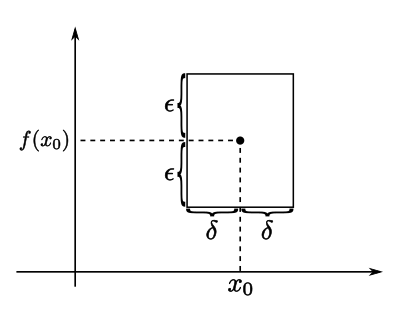
\includegraphics[scale=0.5]{deltaepsilonkrit}
\someshorttext

\begin{wrapfigure}{l}{0.5\textwidth} %this figure will be at the right
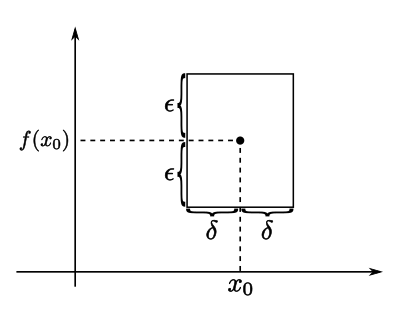
\includegraphics[width=5cm, height=3cm]{deltaepsilonkrit}
\caption{Links, halbe textbreite}
\end{wrapfigure}

\sometext 

\begin{center}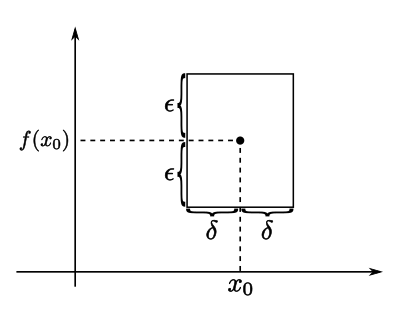
\includegraphics[width=5cm, angle=45]{deltaepsilonkrit}\end{center}

\someshorttext

\begin{figure}[t]
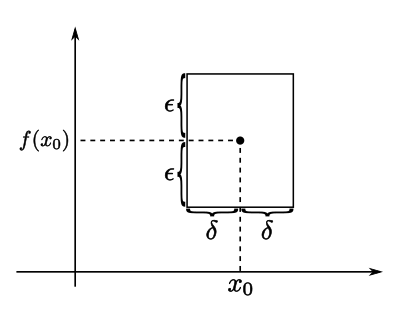
\includegraphics[width=8cm]{deltaepsilonkrit}
\caption{ t -> Top, h -> Here, b -> bottom, p -> special page, ! -> zwingen, H -> precisely at position äquivalent zu h!}
\end{figure}

\sometext

\begin{wrapfigure}{r}{0.25\textwidth} %this figure will be at the right
\centering
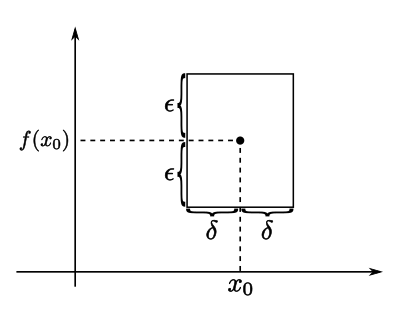
\includegraphics[width=0.25\textwidth]{deltaepsilonkrit}
\caption{Example of a parametric plot ($\sin (x), \cos(x), x$)}
\label{fig:mesh1}    
\end{wrapfigure}

\someshorttext[Abbildung \ref{fig:mesh1}]

\section{Zeichnungen}
\begin{figure}
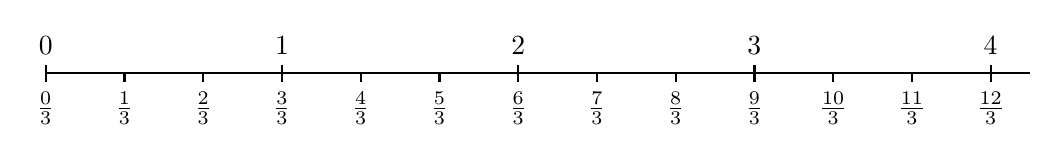
\begin{tikzpicture}[thick]
\newline
    \draw(0,0)--(12.5,0);
    \foreach \x/\xtext in {0/0,3/1,6/2,9/3,12/4}
      \draw(\x,0pt)--(\x,3pt) node[above] {\xtext};
    \foreach \x in {0,1,...,12}
      \draw(\x,0pt)--(\x,-3pt) node[below] {$\frac{\x}{3}$};
  \end{tikzpicture}
\end{figure}

\begin{center}
\begin{tikzpicture}
        \draw[step=1,help lines,black!0] (-1,-1) grid (4,4);
        \draw[->] (-0.5,0) -- (3.5,0)  node[below right] {$Re(z)$};
        \draw[->] (0,-0.5) -- (0,3.5)  node[above left]{$Im(z)$};
        \foreach \Point/\PointLabel in {(0,1)/{\im}, (1,0)/1, (2.21,1.75)/{z=(a,b)}}
        \draw[fill=black] \Point circle (0.05) node[above right] {$\PointLabel$};
        \foreach \Point/\PointLabel in {(2.21,0)/a, (0,1.75)/b}
        \draw \Point circle (0.05) node[above right] {$\PointLabel$};
\end{tikzpicture}
\end{center}

 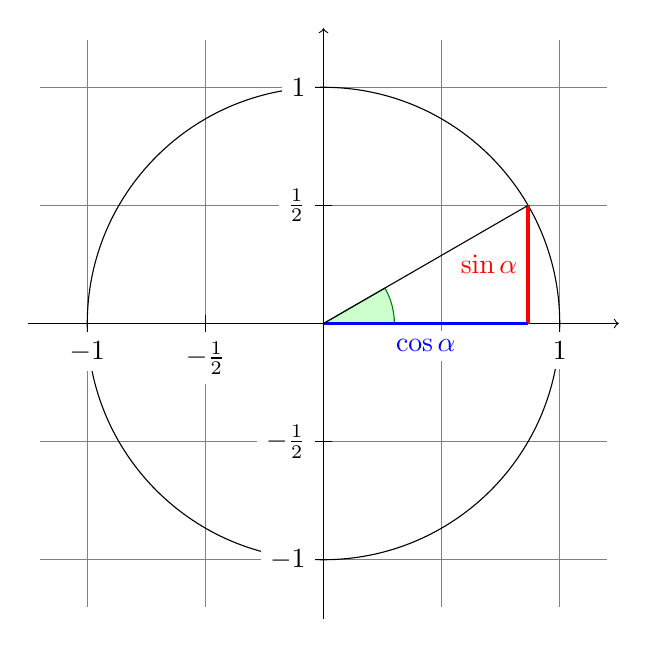
\begin{tikzpicture}[scale=3]
 \draw[step=.5cm, gray, very thin] (-1.2,-1.2) grid (1.2,1.2); 
 \filldraw[fill=green!20,draw=green!50!black] (0,0) -- (3mm,0mm) arc (0:30:3mm) -- cycle; 
 \draw[->] (-1.25,0) -- (1.25,0) coordinate (x axis);
 \draw[->] (0,-1.25) -- (0,1.25) coordinate (y axis);
 \draw (0,0) circle (1cm);
 \draw[very thick,red] (30:1cm) -- node[left,fill=white] {$\sin \alpha$} (30:1cm |- x axis);
 \draw[very thick,blue] (30:1cm |- x axis) -- node[below=2pt,fill=white] {$\cos \alpha$} (0,0);
 \draw (0,0) -- (30:1cm);
 \foreach \x/\xtext in {-1, -0.5/-\frac{1}{2}, 1} 
   \draw (\x cm,1pt) -- (\x cm,-1pt) node[anchor=north,fill=white] {$\xtext$};
 \foreach \y/\ytext in {-1, -0.5/-\frac{1}{2}, 0.5/\frac{1}{2}, 1} 
   \draw (1pt,\y cm) -- (-1pt,\y cm) node[anchor=east,fill=white] {$\ytext$};
 \end{tikzpicture}

\end{document}

